\documentclass[12pt, letterpaper]{article}
%\documentclass[12pt, letterpaper, titlepage]{article}

\usepackage{amsmath}
\usepackage{booktabs}
\usepackage{amsthm}
\usepackage{graphicx}
\usepackage[margin=1in]{geometry}
\usepackage{hyperref}
\hypersetup{colorlinks = true, linkcolor = blue, citecolor=blue, urlcolor = blue}
\usepackage{natbib}
\usepackage{enumitem}
\usepackage{setspace}

\usepackage[]{lineno}
\linenumbers*[1]
% %% patches to make lineno work better with amsmath
\newcommand*\patchAmsMathEnvironmentForLineno[1]{%
 \expandafter\let\csname old#1\expandafter\endcsname\csname #1\endcsname
 \expandafter\let\csname oldend#1\expandafter\endcsname\csname end#1\endcsname
 \renewenvironment{#1}%
 {\linenomath\csname old#1\endcsname}%
 {\csname oldend#1\endcsname\endlinenomath}}%
\newcommand*\patchBothAmsMathEnvironmentsForLineno[1]{%
 \patchAmsMathEnvironmentForLineno{#1}%
 \patchAmsMathEnvironmentForLineno{#1*}}%

\AtBeginDocument{%
 \patchBothAmsMathEnvironmentsForLineno{equation}%
 \patchBothAmsMathEnvironmentsForLineno{align}%
 \patchBothAmsMathEnvironmentsForLineno{flalign}%
 \patchBothAmsMathEnvironmentsForLineno{alignat}%
 \patchBothAmsMathEnvironmentsForLineno{gather}%
 \patchBothAmsMathEnvironmentsForLineno{multline}%
}

% control floats
\renewcommand\floatpagefraction{.9}
\renewcommand\topfraction{.9}
\renewcommand\bottomfraction{.9}
\renewcommand\textfraction{.1}
\setcounter{totalnumber}{50}
\setcounter{topnumber}{50}
\setcounter{bottomnumber}{50}

\newcommand{\jy}[1]{\textcolor{blue}{JY: #1}}
\newcommand{\eds}[1]{\textcolor{red}{EDS: (#1)}}

% NOTE: To produce blinded version, replace "0" with "1" below.
\newcommand{\blind}{0}


%\title{On Misuses of the Kolmogorov--Smirnov Test for One-Sample Goodness-of-Fit}
%
%\author{Anthony Zeimbekakis\\
%%   \href{mailto:anthony.zeimbekakis@uconn.edu}
%% {\nolinkurl{anthony.zeimbekakis@uconn.edu}}\\
  %Elizabeth D.  Schifano\\
  %Jun Yan\\[1ex]
  %Department of Statistics, University of Connecticut\\
%}
%\date{}

\begin{document}
%\maketitle

\if0\blind
{
  \title{\bf On Misuses of the Kolmogorov--Smirnov Test for One-Sample 
	Goodness-of-Fit}
  \author{Anthony Zeimbekakis, %\\
%   \href{mailto:anthony.zeimbekakis@uconn.edu}
% {\nolinkurl{anthony.zeimbekakis@uconn.edu}}\\
  Elizabeth D. Schifano, %\\
  Jun Yan\\[1ex]
  Department of Statistics, University of Connecticut\\
}
\date{}
  \maketitle
} \fi

\if1\blind
{
  \bigskip
  \bigskip
  \bigskip
  \begin{center}
    {\LARGE\bf On Misuses of the Kolmogorov--Smirnov Test for One-Sample 
	Goodness-of-Fit}
\end{center}
  \bigskip
} \fi


\doublespace

\begin{abstract}
The Kolmogorov--Smirnov (KS) test is widely employed to assess the
goodness-of-fit of a hypothesized continuous distribution to a sample.
Despite its popularity, the test is frequently misused in the literature and
practice. While originally intended for independent, continuous data with
precisely specified hypothesized distributions, it is erroneously applied to
scenarios with dependent, discrete, or rounded data, with hypothesized
distributions requiring estimated parameters. For example, it has been
``discovered'' multiple times that the test is too conservative when the 
hypothesized distribution has parameters that need to be estimated.
We demonstrate misuses of the one-sample KS test in
three scenarios through simulation studies:
1) the hypothesized distribution has unspecified parameters;
2) the data are serially dependent; and
3) a combination of the first two scenarios.
For each scenario, we provide remedies for practical applications using
appropriate bootstrap approaches.
The whole demonstration can be used as hands-on education materials on both
goodness-of-fit tests and bootstrap.

\bigskip
\noindent{\sc Keywords}:
nonparametric bootstrap;
parametric bootstrap;
working dependence.
\end{abstract}

%\doublespace

\section{Introduction}
\label{sec:intro}

The Kolmogorov-Smirnov (KS) test is one of the most popular goodness-of-fit
tests for comparing a sample with a hypothesized parametric distribution.
Let $X_1, ..., X_n$ be a random sample of size~$n$ from a continuous
distribution. The null hypothesis $H_0$ is that $X_i$'s follow distribution~$F$.
Let $F_n(t) = \sum_{i=1}^n I(X_i \le t) / n$ be the empirical cumulative
distribution function of the sample, where $I(\cdot)$ is the indicator
function. The KS test statistic is
\begin{equation}
  \label{eq:ks_standard}
  D_n = \sqrt{n} \sup_x | F_{n}(x) - F(x) |.
\end{equation}
The asymptotic distribution of $D_n$ under $H_0$ is independent of the
distribution~$F$. As $n \to \infty$, $D_n$ converges in distribution to
the supremum of standard Brownian bridge \citep{kolmogorov1933sulla}. For large
samples, the tests can be performed with a table \citep{smirnov1948table}.
Critical values for small samples ($n \le 35$) have also been given
\citep{massey1951kolmogorov}. The KS test is available in popular
statistical software packages, such as function \texttt{ks.test()} in R package
\textsf{stats} \citep{R, marsaglia2003evaluating}.


The standard one-sample KS test applies to independent data with a continuous
hypothesized distribution that is completely specified. In practice, however, it
has often been applied without realizing that one or more of these assumptions
do not hold. For example, \citet{noether1963note} showed the conservativeness of
the KS test when applied to discontinuous distributions. The null distribution
of the KS statistic is no longer distribution-free and depends on the
hypothesized distribution~$F$. Computing the
exact and asymptotic distribution of $D_n$ is challenging. Fortunately, the null
distribution of the KS statistic for discontinuous distributions has been
efficiently addressed by \citet{dimitrova2020computing} with a
companion R package \textsf{KSgeneral}. Although a common misuse of the KS test, 
the issue with discontinuous data is not our focus.


When the hypothesized distribution~$F$ contains unspecified parameters, as is
the case in most goodness-of-fit test settings, the standard KS test is not
applicable. \citet{steinskog2007cautionary} ``discovers'' the change in power
when using fitted parameters and stresses caution in using the KS test in
such ways. In fact, using fitted parameters in place of the true parameters in
the KS test has been long known to yield extremely conservative results
\citep[e.g.,][]{lilliefors1967kolmogorov}. This problem can be solved by
parametric bootstrap \citep{efron1985bootstrap, hall1991two}, where
bootstrap samples of the test statistics are constructed from samples
generated from the fitted hypothesized distribution. A nonparametric bootstrap
solution is not trivial because a nonparametric bootstrap sample of the
observed data has ties, which would not happen for continuous distributions.
\citet{babu2004goodness} derived the bias of the standard nonparametric 
bootstrap and
showed how to correct it. They further noted that both parametric and
nonparametric procedures lead to correct asymptotic levels.


The standard KS test does not apply to stationary yet dependent data either. The
distribution of the KS statistic would have a higher variance for positively
dependent data than that derived when the data are independent because of a
smaller effective sample size. For example, for testing normality,
\citet{durilleul1992lack} demonstrate that a naive application of
the KS statistic is too liberal for medium-to-high positive serial dependence,
and that for negative dependence, the behavior is asymmetrical. For remedies,
\citet{weiss1978modification} provides a procedure that is applicable 
specifically for data
modeled by the second-order auto-regressive (AR) process where the AR parameters
are known. Serial dependence affects the validity of the two-sample KS test too.
In a recent paper on online diagnosis of performance variation in
high-performance computing systems, for example, the authors provided no details
about whether they accounted for serial dependence when applying the two-sample
KS test \citep{tuncer2019online}. After comparing various strategies for dealing
with serial dependence, \citet{lanzante2021testing} concludes that a test based
on Monte-Carlo simulations performed the best.
When additionally the hypothesized distribution contains unknown
parameters, the standard KS test becomes even further inapplicable. 


The contribution of this paper is a demonstration of misuses of the one-sample
KS test in three scenarios and their remedies in practice. Contrary to the
assumptions within the statistics community that anyone familiar with the
relevant literature would not be ``misusing'' the KS test, there is still a
considerable journey ahead in educating students and practitioners from diverse
fields on the proper utilization of the KS test and similar tests. The scenarios
that we consider are where:
1) the hypothesized distribution has unspecified parameters;
2) the data are serially dependent; and
3) a combination of the first two scenarios.
In each scenario, the misuse is performed and the impacts are shown. Then, a
remedy is detailed and performed alongside the misuse to show its positive
effects. Specifically, unspecified parameters are handled by parametric
bootstrap; serial dependence is handled by introducing a working autoregressive
moving average (ARMA) model that preserves the serial dependence for a wide
range of dependence structures.
In order to set up the demonstrations, simulated data are used
throughout. The remedies are also performed on various families of
distributions. An R implementation of the proposed methods will be available
after the paper is published.


The rest of the paper is organized as follows. Section~\ref{sec:fitted}
investigates the scenario where the hypothesized distribution has unspecified
parameters. Both parametric and nonparametric bootstrap are available to fix the
issue. Section~\ref{sec:dependence} investigates the scenario where the data of
the empirical distribution are serially dependent. A bootstrap procedure
employing a working ARMA model to account for dependence is proposed as a
working solution. Section~\ref{sec:fittedwithdependence}
explores the case where a combination of the first two scenarios occurs. An  
adjusted bootstrap procedure is proposed as a working solution in this case.  
Section~\ref{sec:conclusion} concludes with a discussion.


\section{Unspecified Parameters}
\label{sec:fitted}

The null hypothesis of a goodness-of-fit test is often a composite hypothesis
instead of a single hypothesis. That is, the hypothesized distribution is a
family of distributions with unspecified parameters instead of a specific member
in this family. Let $F_\theta$ be a family of distributions indexed by parameter
vector~$\theta$. The null hypothesis is
\[
  H_0: \text{the random sample $X_1, \ldots, X_n$
    comes from a distribution $F_\theta$ for some $\theta$.}
\]
Since $\theta$ is unknown, one would naturally estimate $\theta$ by
$\hat\theta_n$ from, for example, maximum likelihood or methods of moments. The
KS statistic would then be computed as
\begin{equation}
  \label{eq:ks_fitted}
  D_n = \sqrt{n} \sup_x | F_n(x) - F_{\hat\theta_n}(x) |.
\end{equation}
An overly large $D_n$ still indicates evidence to reject~$H_0$. To get the
p-value of the observed $D_n$, however, note that the null distribution is not
the same as that in the standard
case~\eqref{eq:ks_standard}. If the same null distribution were used, one would
be testing a different~$H_0$ that the random sample comes from the specific
member distribution~$F_{\hat\theta_n}$ instead of the family~$F_\theta$.


The consequence of using the wrong null distribution for the KS statistic $D_n$
in~\eqref{eq:ks_fitted} can be illustrated through a simple simulation study. A
random sample $X_1, \ldots, X_n$ was generated from a normal
distribution with both mean and variance parameters set equal to 8 ($N(8,8)$), 
and sample size $n = 200$. The maximum likelihood estimates of the mean and 
variance were used as $\hat\theta_n$. The p-value of the test
statistic~$D_n$ in Equation~\eqref{eq:ks_fitted} was obtained by naively calling 
the \texttt{ks.test()} function in~R with the fitted normal distribution as the
hypothesized distribution. That is, the hypothesized distribution was
$N(\bar X, s^2)$ where $\bar X$ is the sample mean and $s^2$ is the sample
variance (with $n$ in the denominator). This experiment was repeated 1000 times
and the probability-probability plot (PP-plot) of the 1000 p-values are 
displayed in the top left plot of Figure~\ref{fig:pp_f}. If the test were
valid, the p-values would be uniformly distributed in the unit
interval and the points in the PP-plot would fall along the diagonal line. 
Clearly, the distribution of the 1000 p-values is very different from what
one would expect to see from 1000 draws from the standard uniform
distribution.  


\begin{figure}[tbp]
  \centering
  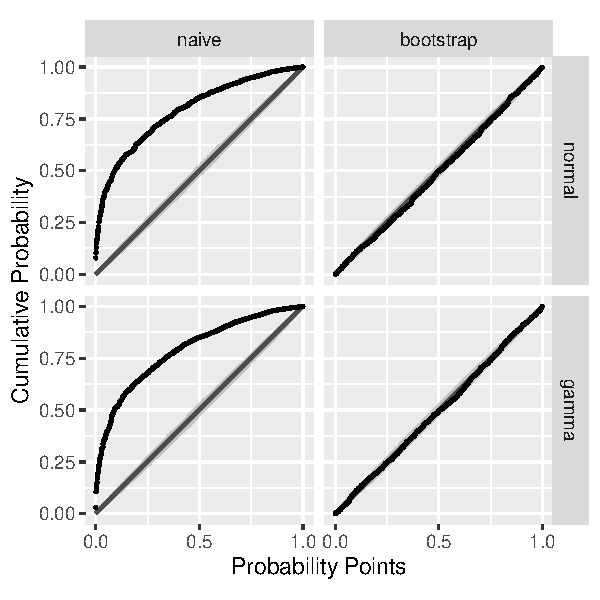
\includegraphics[width=.5\textwidth]{pp_f.pdf}
  \caption{PP-plots for the p-values obtained from KS tests with unspecified
    parameters with sample size $n = 200$ based on 1000 replicates. The data
    generating models were $N(8, 8)$ and $\Gamma(8, 1)$.
  }
  \label{fig:pp_f}
\end{figure}


We similarly considered random samples $X_1, \ldots, X_n$ 
generated from a gamma distribution with shape and scale parameters 8 and 1, 
respectively ($\Gamma(8,1)$), and sample size $n=200$. These parameter values 
were selected so that the mean and variance of the normal and gamma distributions 
in the simulations are the same. Likewise, the p-value of the test 
statistic~$D_n$ in~\eqref{eq:ks_fitted} was obtained by naively calling the
\texttt{ks.test()} function in~R with the fitted gamma distribution as the
hypothesized distribution using the shape and scale maximum likelihood 
estimates. The PP-plot of the p-values from 1000 replications of this 
experiment are displayed in the bottom left plot of Figure~\ref{fig:pp_f}. The
p-values are again non-uniformly distributed due to the use of the 
estimated parameters when specifying the null distribution.


To fix the problem, parametric bootstrap can be used to approximate the null
distribution of the test statistic~$D_n$:
\begin{enumerate}
\item
  Draw a random sample $X_1^*,...,X_n^*$ from the fitted distribution
  $F_{\hat\theta_n}$
\item
  Fit $F_\theta$ to $X_1^*,...,X_n^*$ and obtain estimate 
	$\hat\theta_n^*$ of $\theta$.
\item
  Obtain the empirical distribution function $F_n^*$ of
  $X_1^*, \ldots,  X_n^*$.
\item
  Calculate bootstrap KS statistic
  \[
    D_n^* = \sqrt{n} \sup_x | F_n^* (x)- F_{\hat\theta_n^*}(x) |.
  \]
\item
  Repeat the previous steps a large number~$B$ times and use the empirical
  distribution of $D_n^*$ to approximate the null distribution of the observed
  statistic.
\end{enumerate}
The p-value of $D_n$ is approximated by the proportion of the $D_n^*$ 
statistics that are greater than or equal to~$D_n$.


In the same simulation study, p-values were obtained for the 1000 replicates
from the parametric bootstrap procedures. The top and bottom right plots of 
Figure~\ref{fig:pp_f} display the PP-plots of the 1000
p-values from the normal and gamma data generation scenarios,
respectively. This time, all points fall along the diagonal lines implying that
the p-values are coming from standard uniform distributions.


Nonparametric bootstrap can also be used to approximate the null distribution
of the test statistic in~\eqref{eq:ks_fitted} except that a bias correction is 
needed \citep{babu2004goodness}; see details of the procedure
in the Appendix. The results from nonparametric bootstrap are similar to those
from the parametric bootstrap and, hence, are omitted.


\section{Serially Dependent Data}
\label{sec:dependence}

Here we consider the situation where the observed data $X_1, \ldots, X_n$ are
not independent but serially dependent, and the hypothesized distribution $F$
contains no unknown parameters. That is,
\[
H_0: \text{$X_i$'s have marginal distribution $F$.}
\]
The KS statistic $D_n$ in Equation~\eqref{eq:ks_standard}
is still a good measure of deviation from the null hypothesis. Nonetheless, the
null distribution changes when there is serial dependence.
When the serial dependence is
positive, the effective sample size is less than~$n$. The test statistic
would be stochastically greater than that obtained from independent data, 
resulting in a test that is too liberal (i.e., the null hypothesis is rejected
more often than it should). The reasoning is similar when the serial dependence 
is negative, in which case, the test is conservative.


\begin{figure}[tbp]
  \centering
  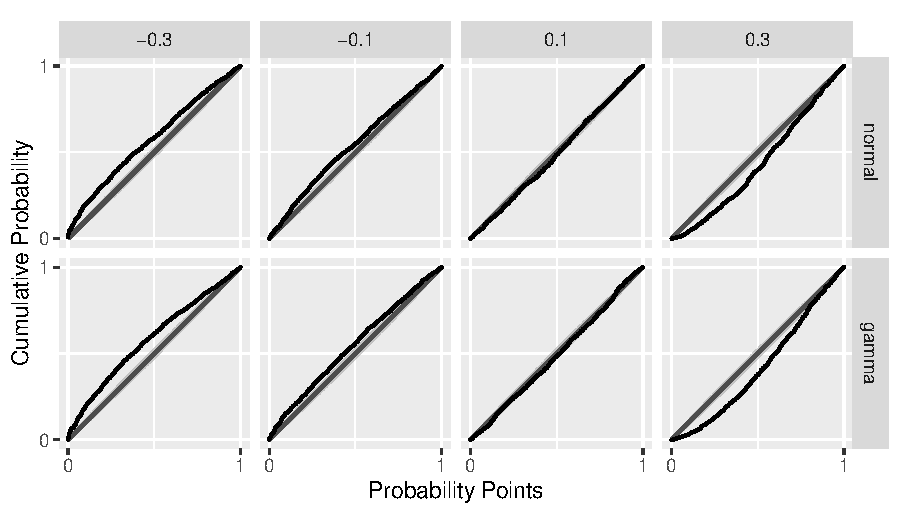
\includegraphics[width=\textwidth]{pp_s.pdf}
  \caption{PP-plots for the p-values obtained from KS test with serial
    dependence ignored and sample size $n = 200$ based on 1000
    replicates. The data have marginal distributions $N(8, 8)$ and
    $\Gamma(8, 1)$, with an AR(1) dependence structure on the standard normal
    scale. The AR coefficients are $\psi \in \{-0.4, -0.2,  0.2,  0.4\}$.
  }
  \label{fig:pp_s}
\end{figure}


The invalidity of the standard statistic for serially dependent data can be
illustrated by a simple simulation study. Consider a first-order autoregressive
or AR(1) model with marginal normal (or gamma) distribution. For each AR
coefficient $\psi \in \{-0.4, -0.2, 0.2, 0.4\}$, we generated 1000
series of length 200. For each series, we applied the KS statistic
in~\eqref{eq:ks_standard} to test $H_0$ that the $X_i$'s follow $N(8, 8)$ (or 
$\Gamma(8,1)$) marginally. The PP-plots of the p-values from $1000$ replicates 
for each $\psi$ value are displayed in Figure~\ref{fig:pp_s}. As 
$\psi$ diverges from 0, the p-values look less likely to be generated from a 
standard uniform distributions. Positive $\psi$ values led to p-values with a 
distribution function higher than the standard uniform distribution function as 
there were more smaller p-values than there should be, and hence, 
liberal tests. Negative $\psi$ values led to p-values with a 
distribution function lower than the standard uniform distribution as there 
were more larger p-values than there should be, and hence, conservative tests.


A complete remedy for KS tests with serially dependent data is
challenging. The null distribution depends on the structure of the serial
dependence, which can be arbitrary in practice. A parametric bootstrap procedure
would need to specify a model for the dependence, whereas the primary interest
is to test the marginal distribution of the stationary series. A block
nonparametric bootstrap for stationary data \citep{kunsch1989jackknife} is
tempting, but the counterpart of a bias correction as in
\citet{babu2004goodness} is not available yet. Is there any approach that does
not require full specification of the dependence of the stationary process,
but still gives reasonably satisfactory correction to the size of the KS test in
certain applications?


We propose a semiparametric bootstrap procedure that assumes a working serial
dependence structure which does not need to be correctly specified. The working
serial dependence is introduced through a working ARMA process with the hope to
approximate the true serial dependence as allowed by the working
model. Essentially, this working model covers the most commonly seen dependence
structure characterized by a normal copula \citep{hofert2018elements}, which
separates the dependence structure
of a multivariate distribution from its marginal distributions. 
The parameters of the working normal copula are
estimated from fitting an ARMA model to the
observed data transformed to the standard normal scale.


In particular, let
$Z_i = \Phi^{-1}\{ F(X_i)\}$, $i = 1, \ldots, n$, where $\Phi$ is the distribution
function of the standard normal. Then we fit an ARMA$(p, q)$ model to
$Z_1, \ldots, Z_n$ with AR order $p$ and MA order $q$ selected by the Akaike
Information Criterion (AIC). This can be done with, for example, function
\texttt{auto.arima()} from  R package \texttt{forecast}
\citep{hyndman2008automatic}. Since it is known that the mean of $Z_i$'s is
zero, it is necessary to set the intercept of the ARMA model as zero in the
fitting process. This restriction turned out to be critical from our
investigation; having the intercept estimated does not lead to desired p-value
distributions in the following bootstrap process.
The selected ARMA$(p, q)$ model with fitted
parameters will be used as the working model to generate bootstrap samples with
serial dependence mimicking that in the observed data. The unconditional
variance $\sigma^2$ of the ARMA model with unit innovation variance can be
obtained with function
\texttt{tacvfARMA()} from R package \texttt{ltsa} \citep{mcleod2007algorithms}.


The semiparametric bootstrap procedure is as follows.
\begin{enumerate}
\item
  Generate $Z_1^*, \ldots, Z_n^*$ from the fitted ARMA$(p, q)$ process with
  innovation variance $1 / \sigma^2$ such that the $Z_i$'s are
	marginally standard normal variables.
\item
  Form a bootstrap sample $X_i^* = F^{-1} [\Phi(Z_i^*)]$,  $i = 1, \ldots, n$,
  where $F^{-1}$ is the quantile function of $F$.
\item
  Obtain the empirical distribution function $F_n^*$ of the bootstrap sample
  $X_1^*, \ldots, X_n^*$.
\item
  Calculate bootstrap KS statistic
  \[
    D_n^* = \sup_x \lvert F_n^* (x)- F(x) \rvert.
  \]
\item
  Repeat the previous steps a large number $B$ times and use the empirical
  distribution of the $B$ test statistics to approximate
  the null distribution of the observed statistic.
\end{enumerate}
The p-value of $D_n$ is, again, approximated by the proportion of the $D_n^*$
statistics that are greater than or equal to~$D_n$. 


This process is semiparametric because the dependence structure is specified by
a normal copula determined by an ARMA process with normally distributed errors.
The closer the approximation is to the truth, the better
performance of the size of the KS test. The normal copula of the working ARMA
process provides a wide class of dependence structures.
If the true dependence indeed has an ARMA structure, this method is exact. When
the true dependence is not covered by the ARMA model, the working model may 
still give a reasonable approximation that can
be useful for practical purposes. 

		
\begin{figure}[tbp]
  \centering
  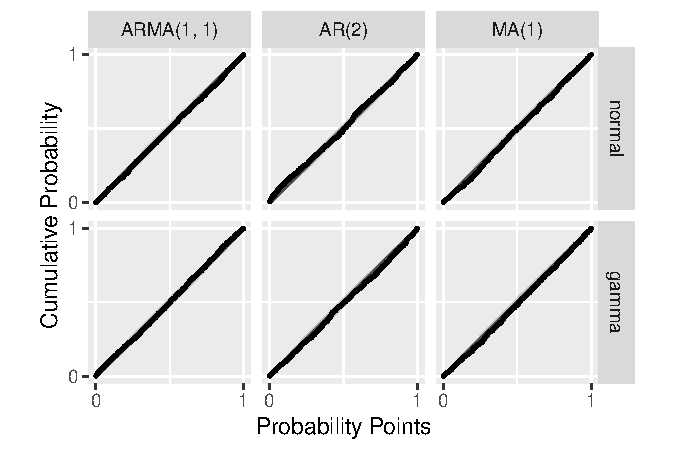
\includegraphics[width=.75\textwidth]{pp_ss.pdf}
  \caption{PP-plots for the p-values obtained from KS test with serial
    dependence accounted for through a working ARMA model and $n = 200$ based on
    1000 replicates. The data have marginal distributions $N(8, 8)$ and
    $\Gamma(8, 1)$. The dependence structure on the standard normal scale was
    characterized by ARMA(1, 1) model, AR(2) model, and MA(1) model.
  }
  \label{fig:pp_ss}
\end{figure}


The semiparametric bootstrap procedure was evaluated in a simulation study. We
considered two marginal distributions: $N(8,8)$ and $\Gamma(8,1)$. Three
dependence structures were used to link variables generated from each marginal
distribution; on the standard normal scale, they are
ARMA(1, 1) with AR coefficient 0.5 and MA coefficient 0.3;
AR(2) with coefficients $(0.6, 0.2)$; and
MA(1) with coefficient 0.8.
For each dependence structure and marginal distribution combination, we
generated 1000 series of length 200.  For each series, we applied the
semiparametric bootstrap procedure with serial
dependence accounted for through a working ARMA model to test $H_0$ that the 
$X_i$'s marginally follow their true marginal distribution ($N(8, 8)$ or 
$\Gamma(8,1)$). Figure~\ref{fig:pp_ss} displays the PP-plots of the 1000 
p-values for each dependence structure and marginal distribution combination.
All plots within the figure show the points falling along the diagonal lines, 
implying that the p-values are coming from standard uniform distributions and 
that the semiparametric bootstrap procedure is an effective remedy in all cases
considered.

\section{Unspecified Parameters and Serially Dependent Data}
\label{sec:fittedwithdependence}

When the observed sample $X_1, \ldots, X_n$ is no longer a random sample but
a serially dependent stationary series, we may still be interested in testing
whether marginally each $X_i$ follows hypothesized distribution with unknown
parameters. That is, the null hypothesis is
\[
H_0: \text{$X_i$'s have marginal distribution $F_\theta$ for some $\theta$}.
\]
The testing statistic $D_n$ in Equation~\eqref{eq:ks_fitted} still measures the
deviation from $H_0$, but its null distribution depends on the serial
dependence. The bootstrap procedure in the last section can be adapted to handle
this situation.


Specifically, let $\hat\theta_n$ be the marginally fitted parameters, and
$Z_i = \Phi^{-1} \{F_{\hat\theta_n}(X_i)\}$, $i = 1, \ldots, n$ be a
transformation of the observed data onto the standard normal scale using the
fitted parameters $\hat\theta_n$. We then fit an ARMA model with orders
selected by the AIC using function \texttt{auto.arima()} from R package
\texttt{forecast}. This ARMA model will be used as the working model to
introduce serial dependence in the bootstrap samples. Again, we obtain the
unconditional variance $\sigma^2$ of the ARMA process with unit innovation
variance. Our semiparametric bootstrap procedure is as follows.

\begin{enumerate}
\item
  Generate $Z_1^*, \ldots, Z_n^*$ from the working ARMA$(p, q)$ model with
  innovation variance $1 / \sigma^2$ such that the $Z_i$'s are marginally
  standard normal variables.
\item
  Form a bootstrap sample
  $X_i^* = F_{\hat\theta_n}^{-1} [\Phi(Z_i^*)]$, $i = 1, \ldots, n$, where
  $F_{\hat\theta_n}^{-1}$ is the quantile function of $F_{\hat\theta_n}$.
\item
  Fit $F_\theta$ to $X_1^*, \ldots, X_n^*$ to obtain estimate $\hat\theta_n^*$
  of $\theta$.
\item
  Obtain the empirical distribution function $F_n^*$ of the bootstrap sample
  $X_1^*, \ldots, X_n^*$.
\item
  Calculate bootstrap KS statistic
  \[
    D_n^* = \sup_x \lvert F_n^* (x) - F_{\hat\theta_n^*} (x) \rvert.
  \]
\item
  Repeat the previous steps a large number $B$ times and use the empirical
  distribution of the $B$ test statistics to approximate
  the null distribution of the observed statistic.
\end{enumerate}
The p-value of $D_n$ is approximated by the proportion of the $D_n^*$
statistics that are greater than or equal to~$D_n$. Compared to the algorithm in
the last section, here we use $F_{\hat\theta_n^*}$ in place of the known~$F$.


\begin{figure}[tbp]
  \centering
  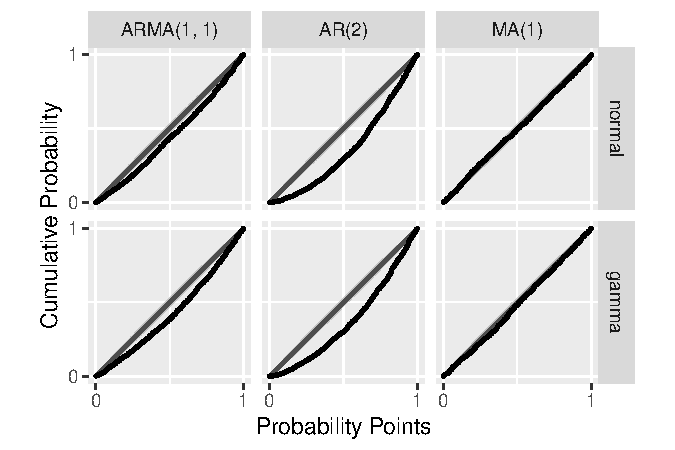
\includegraphics[width=.75\textwidth]{pp_s_f.pdf}
  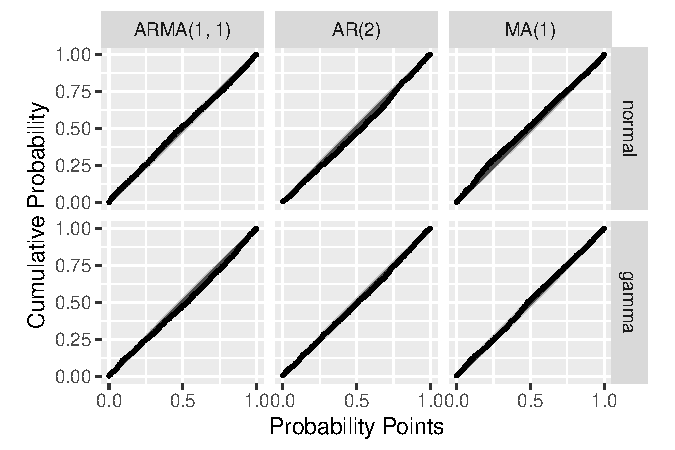
\includegraphics[width=.75\textwidth]{pp_ssf.pdf}
  \caption{PP-plots for the p-values obtained from KS test without (top) and 
	  with (bottom)
    serial dependence accounted for and unspecified parameters; sample size
    $n = 200$ based on
    1000 replicates. The data have marginal distributions $N(8, 8)$ and
    $\Gamma(8, 1)$. The dependence structure on the standard normal scale was
    characterized by ARMA(1, 1) model, AR(2) model, and MA(1) model.
  }
  \label{fig:pp_ssf}
\end{figure}

Figure~\ref{fig:pp_ssf} shows the PP-plots resulting p-values of the
procedure performed on data generated from same simulation settings as in
Section~\ref{sec:dependence}. For comparison, we also displayed the PP-plot of
a naive bootstrap procedure that adjusts for the unspecified parameters as in
Section~\ref{sec:fitted} but not for the serial dependence. 
The super naive approach that does not adjust for fitted parameters nor serial
dependence would have double sin, so the results are not reported. 
The p-values from
naively fitting parameters but not adjusting for dependence clearly deviates
from the standard uniform distribution except in the MA(1) case, where the
autocorrelation is nonzero with a short memory of only lag~1.
Similar to Section~\ref{sec:dependence}, the working normal copula approach
gives p-values with the desired standard uniform distribution regardless of the
true dependence.


\begin{table}[tbp]
  \label{tab:power}
  \caption{Power of rejecting the null hypothesis of normal and gamma
    distribution at significance level 0.05 when the true distribution was
    $\Gamma(8, 1)$ and $N(8, 8)$, respectively. }
\centering
\begin{tabular}{ll cccc}
  \toprule
  &  & \multicolumn{2}{c}{$H_0:$ normal} &
  \multicolumn{2}{c}{$H_0$: gamma}\\
  \cmidrule(lr){3-4}\cmidrule(lr){5-6}
  Dependence & Method & $n = 100$ & $n = 200$ & $n = 100$ & $n = 200$\\
  \midrule
ARMA & naive & 0.404 & 0.656 & 0.515 & 0.779 \\ 
 & copula & 0.330 & 0.556 & 0.442 & 0.722 \\ 
AR & naive & 0.411 & 0.655 & 0.455 & 0.705 \\ 
& copula & 0.261 & 0.448 & 0.313 & 0.544 \\ 
MA & naive & 0.374 & 0.728 & 0.514 & 0.817 \\ 
& copula & 0.343 & 0.693 & 0.487 & 0.797 \\ 
   \bottomrule
\end{tabular}
\end{table}

Finally, we report a small study of the power of the one-sample KS test with
unspecified parameters and serially dependent data. Using the three dependence
models characterized by ARMA(1, 1), AR(2), and MA(1) in the simulation settings
in the last section, we generated serially
dependent data with marginal distributions $N(8, 8)$ left truncated by zero and
$\Gamma(8, 1)$. 
Then, for data from $\Gamma(8, 1)$, we tested $H_0$ that the
data has marginally a normal distribution; for data from $N(8, 8)$ left
truncated by zero, we tested $H_0$ that the data has marginally a gamma
distribution.  In both cases, no parameters were specified. Two sample sizes
were considered, $n \in \{100, 200\}$. Table~\ref{tab:power} summarizes the
power of rejecting the null hypothesis at significance level~0.05 from
1000~replicates. The tests
based on a working copula have substantial power in rejecting the null
hypothesis and the power increases as sample size increases. The power from the
naive tests where the serial dependence is ignored, although the unspecified
parameters are accounted for (i.e., procedure from 
Section~\ref{sec:fitted}), appear to 
have higher power than the proposed tests, but these are not reliable since they 
do not hold their sizes as demonstrated in Figure~\ref{fig:pp_ssf}.


\section{Classroom Implementation}

% Since this is a Teacher's Corner submission, I was hoping to read about how
% these ideas have been presented in specific courses and also how students
% reacted to this. What background did the students have? What level of detail was
% given to them? That is, it is one thing to say "use the bootstrap" and another
% thing to present to students, e.g., a Markdown file with all necessary code
% included. Was that done? Were students invited to conduct their own simulations?
% Etc.

% Graduate level
The misuses of one-sample KS test can be easily incorporated into graduate level
classroom teaching for courses that cover parametric bootstrap. For example, at
the University of Connecticut (UConn), JY has always included a demonstration of
the misuse under unspecified parameters in STAT 5361, Statistical Computing. The
catalog description of this course includes: ``Use of computing for statistical
problems; obtaining features of distributions, fitting models and implementing
inference. Basic numerical methods, nonlinear statistical methods, numerical
integration, modern simulation methods.'' Bootstrap is covered under ``modern
simulation methods.''  The course is open to graduate students in Statistics,
others with permission. Detailed R code and graphical illustrations available in
the open-access course notes elucidate the distinctions between employing null
hypotheses with and without defined parameters (accessible at:
\url{https://jun-yan.github.io/stat-5361/boot.html#parametric-bootstrap}).
Students were able to follow the demonstration closely, gaining a clear
understanding of the implications of using estimated parameters within test
statistics, and learning about the efficacy of the parametric bootstrap method
as a corrective measure.


Supplementary materials accompanying this paper present R code that simplifies
the illustration of the three common misuses of the one-sample KS test in
classrooms, whether during lectures or as part of homework assignments.
Addressing the misuses in contexts of serial dependency necessitates familiarity
with ARMA models in time series analysis---a prerequisite achievable by most
statistics graduate students. While incorporating copulas to model dependency
structures extends beyond conventional statistics curricula, it presents an
opportunity for advanced exploration in courses focused on statistical computing
or multivariate analysis. 


% Undergraduate level (could mention AZ's undergraduate thesis)
At the undergraduate level, so far only the misuses of one-sample KS test have 
been presented and demonstrated in a classroom setting. At UConn, ES 
incorporated this material in STAT 3215, Applied Linear Regression in Data 
Science, as the one-sample KS test is used in residual diagnostics for testing 
whether the externally studentized residuals can be viewed as realizations of a 
standard normal distribution for large samples. %The catalog description of this 
%course states the following topics: ``Applied multiple 
%linear regression analysis in data science, with an emphasis on modern 
%statistical regression methods: simple linear regression and correlation 
%analysis, multiple linear regression, analysis of variance, goodness of fit, 
%comparing regression models through partial and sequential F tests, dummy 
%variables, regression assumptions and diagnostics, model selection and penalized 
%regression, prediction and model validation, principles of design of experiments, 
%one-way and two-way analysis of variance.'' 
Students in this applied linear regression course are required
to have taken either two semesters of introductory statistics or a 
Calculus~2-based statistical methods course as a prerequisite. In the KS 
assignment, students were introduced to a more detailed description of the KS 
test, and were provided R code and output for a simulation study that showed  
KS test performance (in terms of the distribution of $p$-values) under a 
scenario where all KS test assumptions were met (independent, continuous data 
with precisely specified hypothesized distributions). When the scenario was 
modified to use estimated parameters instead, the students were asked modify the 
previous simulation code and show the resulting distribution of $p$-values. The 
assignment is included in the Supplemental Materials. 

While students in this course are exposed to the bootstrap in the 
context of linear regression models (specifically, case resampling and residual 
bootstrap), they are not in general familiar with serially dependency. Thus, the 
remedies and more complicated serially dependent settings were not presented in 
the undergraduate applied linear regression course. Serial dependence is covered 
in other undergraduate courses, and in fact, the contents of this manuscript 
were the basis of AZ's undergraduate honors thesis. Consequently, all 
statistical concepts and methods employed within this paper are certainly within 
reach of many UConn undergraduate Statistics and Statistical Data Science 
majors.     

\section{Concluding Remarks}
\label{sec:conclusion}

The three kinds of misuses of the KS test for one-sample goodness-of-fit that we
demonstrated here are commonly seen in practice. With the aid of computing tools
such as R, they can be easily demonstrated in classroom teaching. Practitioners
need to be aware of the assumptions of the standard one-sample KS test that the
hypothesized distribution is completely specified and that the data are
independent. When these assumptions are not met, naive applications of the test
are no longer accurate and remedies must be performed. In the
case of fitted parameters, parametric and nonparametric bootstrap can restore
the size of the test. The nonparametric version has long been developed too but
is lesser known \citep{babu2004goodness}. In the case of serially dependent data,
our semiparametric bootstrap procedure with a working dependence structure
controlled by an automatically selected ARMA model restores the size of the test
for a wide range of dependence structures.
When both assumptions are violated, i.e., where the data has serial 
dependence and the parameters must be fitted, a combination of the two
individual remedies shows good results. The misuses of the KS test also apply
to other goodness-of-fit tests based on the empirical distribution
function, such as the Anderson--Darling test or the Cramér-—von Mise test, which
are known to be superior to KS in certain respects \citep{stephens2017tests}.
Similar bootstrap remedies can be developed for these tests.


The semiparametric bootstrap procedure with a working ARMA dependence structure
is not a complete solution and has limitations. When the true serial dependence
can be well approximated by an ARMA model, the model selection process could be
replaced with
autoregressive sieve, i.e., a sequence of autoregressive models the order of 
which increases
simultaneously with the sample size although at a suitably slower rate 
\citep[e.g.,][]{psaradakis2017distance, psaradakis2020normality}.
When the true serial dependence
structure cannot be well approximated by an ARMA model with normally distributed
error terms, the remedy may not restore the size of the test. The working
dependence structure is essentially the normal copula uniquely determined by the
ARMA model with normal errors. Some copulas are quite different from the normal
copula. For example, extreme value copulas have tail dependence, which is not
provided by normal copulas.
Using a normal copula to approximate an extreme value copula may not capture the
true serial dependence structure that is needed to restore the size of the
test. A block version of the nonparametric bootstrap \citep{babu2004goodness},
which avoids specification of a working dependence structure, would be more
desirable.


Statisticians living in
an ivory tower tend to doubt that anyone would be misusing the KS test as we
illustrated given that such situations are very well-known in the statistics
literature. It is our experience, however, that much effort is needed in
propagating many knowns in the statistics community to the real wild world
through innovative and impactful education. Such effort may be more valuable
than developing more advanced methods that few people would use in practice.


\section*{Data Availability Statement}
An R implementation of the proposed methods will be made publicly available upon 
publication.

\appendix

\section{Appendix: Nonparametric Bootstrap for KS Test with Fitted Parameters}

Using the same notations in the text, the nonparametric bootstrap procedure 
is summarized as follows \citep{babu2004goodness}.
\begin{enumerate}
\item
  Draw a random sample $X_1^*,...,X_n^*$ from the empirical distribution $F_n$
  with replacement.
\item
  Fit $F_\theta$ to $X_1^*,...,X_n^*$ and obtain estimate 
	$\hat\theta_n^*$ of $\theta$.
\item
  Obtain the empirical distribution function $F_n^*$ of
  $X_1^*, \ldots,  X_n^*$. 
\item
  Calculate bootstrap KS statistic
  \[
    D_n^* = \sup_x | \sqrt{n}\left(F_n^* (x)- F_{\hat\theta_n^*}(x)\right) - B_n(x) |.
  \]
  where $B_{n}(x) = \sqrt{n}(F_{n}(x) - F_{\hat\theta_n}(x))$ is the known
  bias term.
\item
  Repeat the previous steps a large number $B$ times and use the empirical
  distribution of $D_n^*$ to approximate the null distribution of the observed
  statistic. 
\end{enumerate}
The p-value of $D_n$ is, again, approximated by the proportion of the $D_n^*$
statistics that are greater than or equal to~$D_n$. Note that the step~1 and
step~4 are different from the parametric bootstrap version.

\bibliographystyle{asa}
\bibliography{citations}


\end{document}
%%% LocalWords: nonparametric semiparametric autocorrelation ARMA
%%% Local Variables:
%%% mode: latex
%%% TeX-master: t
%%% ispell-personal-dictionary: ".aspell.en.pws"
%%% fill-column: 80
%%% eval: (auto-fill-mode 1)
%%% End:
